
\documentclass[10pt]{report}
\usepackage{kvmap}
\usepackage{listings} 
\usepackage{geometry}
\usepackage{tabularx} 
\usepackage[framemethod=tikz]{mdframed}
 \geometry{
 a4paper,
 total={170mm,257mm},
 left=20mm,
 top=20mm,
 }
\usepackage{multicol}
\usepackage {graphicx}
\begin{document}
\centering {
\includegraphics[scale=0.05]{logo.jpg}} \vspace{3mm}\\ \raggedright Name: S.Kedareswari\hspace{12cm}\\
\raggedleft Roll No.: FWC22049
\\ \centering \Large \textbf{ASSIGNMENT-1}\vspace{3mm}\normalsize\\ 
\begin{multicols}{2} 
\section{Design of Xnor Gate using nor gates}

\section{Contents}
\raggedright
\textbf{Components}
\hspace{10em} 3
\\\textbf{Hardware}
\hspace{11.3em}   4
\\\textbf{Solution}
\hspace{12.1em}   5\\
\textit{Abstract-}
\textbf{This manual shows how to design Xnor gate using nor gates}
\section{Components}
\centering
\begin{tabular}{|l|c|c|}
\hline
Component & Value & Quantity\\
\hline
Resistor & 220 Ohm & 1\\
\hline
Arduino & UNO & 1\\
\hline
LED & & 1\\
\hline
Jumper Wires & M-M & 20\\
\hline
Breadboard & & 1\\
\hline
\end{tabular}\\
\
\centerline{Table 3.0}
\section{Xnor Truth Table}
\raggedright

\
\centering
\\\begin{tabular}{|l|c|c|c|c|} \hline
  \textbf{A}& \textbf{B} & \textbf{G(A,B)}\\ \hline
0&0&1\\ \hline
0&1&0 \\ \hline
1&0&0\\ \hline
1&1&1\\ \hline
\end{tabular}\\
\
\section{Circuit Diagram}

\
\raggedleft{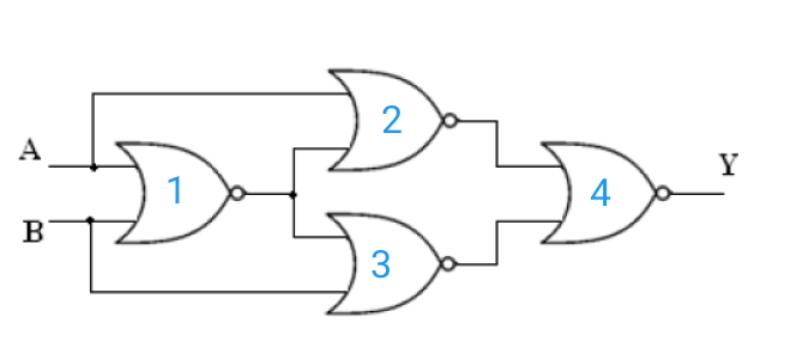
\includegraphics[scale=0.3]{ckt.png}} \vspace{3mm}\\
\

  
  \centering  \section{Boolean Logic}
   \centering  1=(A+B)'\\
   2=(A+x1)'\\ 
   3=(B+x1)'\\
   4=(x2+x3)' \\
   
   \section{Hardware}
   \begin{tabular}{|l|c|c|c|c|c|c|} \hline 
\textbf{Arduino} & \textbf{D13} & \textbf{GND} \\ \hline
\textbf{Led} & \textbf{+VE} & \textbf{-VE}\\ \hline
\end{tabular} \\
\ 
\centerline{Table 7.0}
   
 \section{Hardware Connection}
  \raggedright
  Give the connections as per Table 3. For taking the inputs connect 5V of arduino to +ve line of bread board to consider it as logic 'HIGH'.Connect GND pin of arduino to -ve line of bread board to consider it as logic 'LOW'.\\
For example if the inputs A,B are connected 1,0 respectively the output should be 0 i.e., the LED connected to the 2nd pin should turn off.
\\
In the another case if we connect the inputs A,B to 1,1 respectively the output should be 1 i.e., the LED connected to 2nd pin should glow

\section{Software}
  1.Connect the arduino to the USB port of computer
  \\
  2.Download the follwing code
  \begin{lstlisting}
     https://github.com/kedareswari200/fwc
     -module1/blob/main/assi1_assembly/assem.asm
  \end{lstlisting}
  
  3.Upload the code into the arduino board.
  \\
  4.The output '1' is represented as the state:'LED ON' and '0' is represented as the state 'LED OFF'

\end{multicols}
\end{document}